\documentclass[a4paper,12pt,oneside,article]{memoir}
\setlrmarginsandblock{3cm}{*}{1}
\setulmarginsandblock{3cm}{*}{1}
\setheadfoot{2cm}{\footskip}          
\checkandfixthelayout[nearest]


\setlength{\parindent}{0pt}

\usepackage[utf8]{inputenc} % 显示中文
\usepackage{fancyhdr} % 导入fancyhdr包
\usepackage{amsmath, amssymb, bm, mathtools, mathdots}

\pagestyle{fancy}
% 页眉设置
\fancyhf{}
\fancyhead[L]{Yilin Chen}
\fancyhead[R]{\today}
\fancyhead[C]{\rightmark}
% 页脚设置
\fancyfoot[L]{Powered by \LaTeX}
\fancyfoot[C]{\thepage} % 页码
\fancyfoot[R]{DM Homework Assignment}
\renewcommand{\headrulewidth}{4pt} % 分隔线宽度4磅
\renewcommand{\footrulewidth}{2pt}

\usepackage{newtxtext}
\usepackage{geometry}
\usepackage[dvipsnames,svgnames]{xcolor}
% \usepackage[strict]{changepage} % 提供一个 adjustwidth 环境
%\usepackage{framed} % 实现方框效果
\usepackage{tcolorbox}
\usepackage{float}
\usepackage{shortlst}
\usepackage{makecell}
\usepackage{graphicx}
\usepackage{caption}

\setcounter{secnumdepth}{0}

\definecolor{formalshade}{rgb}{0.95,0.95,1} % 文本框颜色
\definecolor{greenshade}{rgb}{0.90,0.99,0.91} % 绿色文本框,竖线颜色设为 Green
\definecolor{redshade}{rgb}{1.00,0.90,0.90}% 红色文本框,竖线颜色设为 LightCoral
\definecolor{brownshade}{rgb}{0.99,0.97,0.93} % 莫兰迪棕色,竖线颜色设为 BurlyWood

\newenvironment{formal}{%
\def\FrameCommand{%
\hspace{1pt}%
{\color{DarkBlue}\vrule width 2pt}%
{\color{formalshade}\vrule width 4pt}%
\colorbox{formalshade}%
}%

\MakeFramed{\advance\hsize-\width\FrameRestore}%
\noindent\hspace{-4.55pt}
\begin{adjustwidth}{}{7pt}%
\vspace{2pt}\vspace{2pt}%
}
{%
\vspace{2pt}\end{adjustwidth}\endMakeFramed%
}

\usepackage[framemethod=TikZ]{mdframed}

\newcounter{Sol}[section]
\renewcommand{\theSol}{\arabic{section}.\arabic{Sol}}
\newenvironment{Sol}[1][]{
	\refstepcounter{Sol}
	\mdfsetup{
		frametitle={
			\tikz[baseline=(current bounding box.east), outer sep=0pt]
			\node[anchor=east,rectangle,fill=blue!20]
			{\strut Solution~\ifstrempty{#1}{}{:~#1}};},
		innertopmargin=10pt,linecolor=blue!20,
		linewidth=2pt,topline=true,
		frametitleaboveskip=\dimexpr-\ht\strutbox\relax
	}
	\begin{mdframed}[]\relax
}{\end{mdframed}}


\begin{document}
\chapter*{Chapter 1 The Foundations:Logic and Proofs}
\section{1.1 Propositional Logic}

%---------------------------------------------------------------------------
	\begin{tcolorbox}
		[colback=Emerald!10,colframe=cyan!40!black,title=\textbf{Question 11}]
		Let \textit{p} and \textit{q} be the propositions ``Swimming at the New Jerssey shore is allowed'' and ``Sharks have been spotted near the shore,'' respectively. Express each of these compound propositions as an English sentence.\\

		\begin{shortenumerate}[a]
			\item $\lnot \textit{q} $
			\item $\textit{p}\land \textit{q} $
			\item $\lnot \textit{p}\lor \textit{q} $
			\item $\textit{p}\rightarrow \lnot \textit{q} $
			\item $\lnot \textit{q} \rightarrow \textit{p}$
			\item $\lnot \textit{p}\rightarrow \textit{q} $
			\item $\textit{p}\leftrightarrow \lnot \textit{q} $
			\item $\lnot \textit{p}\land (\textit{p}\lor \lnot \textit{q} )$
		\end{shortenumerate}
	\end{tcolorbox}
	\begin{Sol}[]
		\begin{enumerate}[1]
			\item Sharks have \textbf{not} been spotted near the shore
			\item Swimming at the New Jerssey shore is allowed \textbf{and} sharks have been spotted near the shore 
			\item Swimming at the New Jerssey shore is \textbf{not} allowed or sharks have been spotted near the shore
			\item \textbf{If} swimming at the New Jerssey shore is allowed \textbf{then} sharks have \textbf{not} been spotted near the shore
			\item \textbf{If} sharks have \textbf{not} been spotted near the shore, \textbf{then} swimming at the New Jerssey shore is allowed 
			\item \textbf{If} swimming at the New Jerssey shore is \textbf{not} allowed, sharks have been spotted near the shore
			\item \textbf{If and only if} swimming at the New Jerssey shore is allowed, \textbf{then} sharks have \textbf{not} been spotted near the shore
			\item Swimming at the New Jerssey shore is \textbf{not} allowed, \textbf{but} swimming at the New Jerssey shore is allowed \textbf{or} sharks have \textbf{not} been spotted near the shore
		\end{enumerate}
	\end{Sol}
%---------------------------------------------------------------------------

\clearpage	

%---------------------------------------------------------------------------

	\begin{tcolorbox}
		[colback=Emerald!10,colframe=cyan!40!black,title=\textbf{Question 17}]
		Let \textit{p}, \textit{q}, and \textit{r} be the propositions

		\begin{flushleft}
			\hspace*{1cm} \textit{p}: Grizzly bears have been seen in the area. \\
			\hspace*{1cm} \textit{q}: Hiking is safe on the trail. \\
			\hspace*{1cm} \textit{r}: Berries are ripe along the trail. \\
		\end{flushleft}

		Write these propositions using \textit{p}, \textit{q}, and \textit{r} and logical connectives (including negations).	

		\begin{enumerate}[a)]
			\item Berries are ripe along the trail, but grizzly bears have not been seen in the area.
			\item Grizzly bears have not been seen in the area and hiking on the trail is safe, but berries are ripe along the trail.
			\item If berries are ripe along the trail, hiking is safe if and only if grizzly bears have not been seen in the area.
			\item It is not safe to hike on the trail, but grizzly bears have not been seen in the area and the berries along the trail are ripe.
			\item For hiking on the trail to be safe, it is necessary butnot sufficient that berries not be ripe along the trail and for grizzly bears not to have been seen in the area
			\item Hiking is not safe on the trail whenever grizzly bears have been seen in the area and berries are ripe along the trail.
		\end{enumerate}
	\end{tcolorbox}
	\begin{Sol}[]
		\begin{enumerate}[a)]
			\item $r \land \lnot p$
			\item $(\lnot p \land q) \land r$ 
			\item $r\rightarrow (q \leftrightarrow \lnot p)$
			\item $\lnot q\land (\lnot p \land r)$
			\item $q \rightarrow( \lnot r \land \lnot p)$
			\item $\lnot q \leftarrow (p \land r)$
		\end{enumerate}
	\end{Sol}
%---------------------------------------------------------------------------

\clearpage

%---------------------------------------------------------------------------

\begin{tcolorbox}
	[colback=Emerald!10,colframe=cyan!40!black,title=\textbf{Question 24}]
	Write each of these statements in the form ``if \textit{p}, then \textit{q}'' in English. [\textit{Hint}: Refer to the list of common ways to express conditional statements provided in this section.]
	\begin{enumerate}[a)]
		
		\item It is necessary to wash the boss`s car to get promoted.
		\item Winds from the south imply a spring thaw.
		\item A sufficient condition for the warranty to be good is that you bought the computer less than a year ago.
		\item Willy gets caught whenever he cheats.
		\item You can access the website only if you pay a subscription fee.
		\item Getting elected follows from knowing the right people
		\item Carol gets seasick whenever she is on a boat.
	\end{enumerate}
\end{tcolorbox}
\begin{Sol}[]
	\begin{enumerate}[a)]
		\item \textbf{If} you get promoted, \textbf{then} the boss`s car is washed.
		\item \textbf{If} winds from the south, \textbf{then} a spring thaw
		\item \textbf{If} you bought the computer less than a year ago, \textbf{then} the warranty is good.
		\item \textbf{If} Willy cheats, \textbf{then} Willy gets caught.
		\item \textbf{If} you can access the website, \textbf{then} you pay a subscription fee.
		\item \textbf{If} knowing the right people, \textbf{then} getting elected.
		\item \textbf{If} Carol is on a boat, \textbf{then} Carol gets seasick.
	\end{enumerate}
\end{Sol}
%---------------------------------------------------------------------------

\clearpage

%---------------------------------------------------------------------------

\begin{tcolorbox}
	[colback=Emerald!10,colframe=cyan!40!black,title=\textbf{Question 30}]
	State the converse, contrapositive, and inverse of each of these conditional statements.
	\begin{enumerate}[a)]
		\item If it snows tonight, then I will stay at home.
		\item I go to the beach whenever it is a sunny summer day.
		\item When I stay up late, it is necessary that I sleep until noon.
	\end{enumerate}
\end{tcolorbox}
\begin{Sol}[]
	\begin{enumerate}[a)]
		\item \textit{If it snows tonight, then I will stay at home.}
			\begin{itemize}
				\item \textbf{converse}: If I stay at home, then it will snow tonight.
				\item \textbf{contrapositive}: If I do not stay at home, then it will not snow tonight.
				\item \textbf{inverse}: If it does not snow tonight, then I will not stay at home.
			\end{itemize}
		\item \textit{I go to the beach whenever it is a sunny summer day.}
			\begin{itemize}
				\item \textbf{converse}: It is a sunny summer day whenever I go to the beach.
				\item \textbf{contrapositive}: It is not a sunny summer day whenever I do not go to the beach.
				\item \textbf{inverse}: I do not go to the beach whenever it is not a sunny summer day.
			\end{itemize}
		\item \textit{When I stay up late, it is necessary that I sleep until noon.}
			\begin{itemize}
				\item \textbf{converse}: When I sleep until noon, it is necessary that I stay up late.
				\item \textbf{contrapositive}: When I do not sleep until noon, it is necessary that I do not stay up late.
				\item \textbf{inverse}: When I do not stay up late, it is necessary that I would not sleep until noon.
			\end{itemize}
	\end{enumerate}
\end{Sol}
%---------------------------------------------------------------------------

\clearpage

%---------------------------------------------------------------------------
\begin{tcolorbox}
	[colback=Emerald!10,colframe=cyan!40!black,title=\textbf{Question 33}]
	Construct a truth table for each of these compound propositions.
	\begin{enumerate}[a)]
		\item $p \land \lnot p $
		\item $p \lor \lnot p $
		\item $(p \lor \lnot q) \rightarrow q $
		\item $(p \lor q) \rightarrow (p \land q) $
		\item $(p \rightarrow q) \leftrightarrow (\lnot q \rightarrow \lnot p) $
		\item $ (p \rightarrow q) \rightarrow (q \rightarrow p) $
	\end{enumerate}
\end{tcolorbox}
\begin{Sol}[]
	\begin{enumerate}[a)]
		\setlength{\itemsep}{1cm}
		\setlength{\parsep}{2pt}
		\item \begin{tabular}{|p{2cm}|p{2cm}|p{4cm}}
					\makecell[c]{$p$} & \makecell[c]{$\lnot p$} & \makecell[c]{$p \land \lnot p $} \\
					\makecell[c]{T}& \makecell[c]{F}& \makecell[c]{F}\\
					\makecell[c]{F}& \makecell[c]{T}& \makecell[c]{F}
			\end{tabular}
		\item \begin{tabular}{|p{2cm}|p{2cm}|p{4cm}}
				\makecell[c]{$p$}& \makecell[c]{$\lnot p$} & \makecell[c]{$p \lor \lnot p $} \\
				\makecell[c]{T}& \makecell[c]{F}& \makecell[c]{T}\\
				\makecell[c]{F}& \makecell[c]{T}& \makecell[c]{T}
			\end{tabular}
		\item \begin{tabular}{|p{2cm}|p{2cm}|p{4cm}}
				\makecell[c]{$p$}& \makecell[c]{$q$} & \makecell[c]{$(p \lor \lnot q) \rightarrow q $} \\
				\makecell[c]{T}& \makecell[c]{T}& \makecell[c]{T}\\
				\makecell[c]{T}& \makecell[c]{F}& \makecell[c]{F}\\
				\makecell[c]{F}& \makecell[c]{T}& \makecell[c]{T}\\
				\makecell[c]{F}& \makecell[c]{F}& \makecell[c]{F}
			\end{tabular}	
		\item \begin{tabular}{|p{2cm}|p{2cm}|p{4cm}}
				\makecell[c]{$p$}& \makecell[c]{$q$} & \makecell[c]{$(p \lor q) \rightarrow (p \land q) $} \\
				\makecell[c]{T}& \makecell[c]{T}& \makecell[c]{T}\\
				\makecell[c]{T}& \makecell[c]{F}& \makecell[c]{F}\\
				\makecell[c]{F}& \makecell[c]{T}& \makecell[c]{F}\\
				\makecell[c]{F}& \makecell[c]{F}& \makecell[c]{T}
			\end{tabular}
		\item \begin{tabular}{|p{2cm}|p{2cm}|p{4cm}}
				\makecell[c]{$p$}& \makecell[c]{$q$} & \makecell[c]{$(p \rightarrow q) \leftrightarrow (\lnot q \rightarrow \lnot p) $} \\
				\makecell[c]{T}& \makecell[c]{T}& \makecell[c]{T}\\
				\makecell[c]{T}& \makecell[c]{F}& \makecell[c]{T}\\
				\makecell[c]{F}& \makecell[c]{T}& \makecell[c]{T}\\
				\makecell[c]{F}& \makecell[c]{F}& \makecell[c]{T}
			\end{tabular}
		\item \begin{tabular}{|p{2cm}|p{2cm}|p{4cm}}
				\makecell[c]{$p$}& \makecell[c]{$q$} & \makecell[c]{$ (p \rightarrow q) \rightarrow (q \rightarrow p) $} \\
				\makecell[c]{T} & \makecell[c]{T} & \makecell[c]{T} \\
				\makecell[c]{T} & \makecell[c]{F}& \makecell[c]{T} \\
				\makecell[c]{F}& \makecell[c]{T} & \makecell[c]{F} \\
				\makecell[c]{F}& \makecell[c]{F}& \makecell[c]{T}
			\end{tabular}		
	\end{enumerate}
\end{Sol}
%---------------------------------------------------------------------------

\clearpage

%---------------------------------------------------------------------------

\begin{tcolorbox}
	[colback=Emerald!10,colframe=cyan!40!black,title=\textbf{Question 34}]
	Construct a truth table for each of these compound propositions.
	\begin{enumerate}[a)]
		\item $p \rightarrow \lnot p $
		\item $p \leftrightarrow \lnot p$
		\item $p \oplus  (p \lor q)$
		\item $(p \land q) \rightarrow (p \lor q)$
		\item $(q \rightarrow \lnot p) \leftrightarrow (p \leftrightarrow q)$
		\item $(p \leftrightarrow q) \oplus (p \leftrightarrow \lnot q)$
	\end{enumerate}
\end{tcolorbox}
\begin{Sol}[]
	\begin{enumerate}[a)]
		\setlength{\itemsep}{1cm}
		\setlength{\parsep}{2pt}
		\item \begin{tabular}{|p{2cm}|p{2cm}|p{4cm}}
					\makecell[c]{$p$} & \makecell[c]{$\lnot p$} &\makecell[c]{$p \rightarrow \lnot p$} \\
					
					\makecell[c]{T}& \makecell[c]{F}& \makecell[c]{T}\\
					\makecell[c]{F}& \makecell[c]{T}& \makecell[c]{T}
				\end{tabular}
		\item \begin{tabular}{|p{2cm}|p{2cm}|p{4cm}}
					\makecell[c]{$p$}& \makecell[c]{$p$} & \makecell[c]{$p \leftrightarrow \lnot p$} \\
					
					\makecell[c]{T}& \makecell[c]{F}& \makecell[c]{F}\\
					\makecell[c]{F}& \makecell[c]{T}& \makecell[c]{F}
				\end{tabular}
		\item \begin{tabular}{|p{2cm}|p{2cm}|p{4cm}}
					\makecell[c]{$p$}& \makecell[c]{$q$} & \makecell[c]{$p \oplus  (p \lor q)$} \\
					\makecell[c]{T}& \makecell[c]{T}& \makecell[c]{F}\\
					\makecell[c]{T}& \makecell[c]{F}& \makecell[c]{F}\\
					\makecell[c]{F}& \makecell[c]{T}& \makecell[c]{T}\\
					\makecell[c]{F}& \makecell[c]{F}& \makecell[c]{F}
				\end{tabular}	
		\item \begin{tabular}{|p{2cm}|p{2cm}|p{4cm}}
					\makecell[c]{$p$}& \makecell[c]{$q$} & \makecell[c]{$(p \land q) \rightarrow (p \lor q)$} \\
					\makecell[c]{T}& \makecell[c]{T}& \makecell[c]{T}\\
					\makecell[c]{T}& \makecell[c]{F}& \makecell[c]{T}\\
					\makecell[c]{F}& \makecell[c]{T}& \makecell[c]{T}\\
					\makecell[c]{F}& \makecell[c]{F}& \makecell[c]{T}
				\end{tabular}
		\item \begin{tabular}{|p{2cm}|p{2cm}|p{4cm}}
					\makecell[c]{$p$}& \makecell[c]{$q$} & \makecell[c]{$(q \rightarrow \lnot p) \leftrightarrow (p \leftrightarrow q)$} \\
					\makecell[c]{T}& \makecell[c]{T}& \makecell[c]{F}\\
					\makecell[c]{T}& \makecell[c]{F}& \makecell[c]{T}\\
					\makecell[c]{F}& \makecell[c]{T}& \makecell[c]{F}\\
					\makecell[c]{F}& \makecell[c]{F}& \makecell[c]{T}
				\end{tabular}
		\item \begin{tabular}{|p{2cm}|p{2cm}|p{4cm}}
					\makecell[c]{$p$}& \makecell[c]{$q$} & \makecell[c]{$(p \leftrightarrow q) \oplus (p \leftrightarrow \lnot q)$} \\
					\makecell[c]{T} & \makecell[c]{T} & \makecell[c]{T} \\
					\makecell[c]{T} & \makecell[c]{F}& \makecell[c]{T} \\
					\makecell[c]{F}& \makecell[c]{T} & \makecell[c]{T} \\
					\makecell[c]{F}& \makecell[c]{F}& \makecell[c]{T}
				\end{tabular}		
	\end{enumerate}
\end{Sol}
%---------------------------------------------------------------------------

\clearpage

%---------------------------------------------------------------------------

\begin{tcolorbox}
	[colback=Emerald!10,colframe=cyan!40!black,title=\textbf{Question 35}]
	Construct a truth table for each of these compound propositions.
	\begin{enumerate}[a)]
		\item $(p \lor q) \rightarrow (p \oplus q) $
		\item $(p \oplus q) \rightarrow (p \land q)$
		\item $(p \lor q) \oplus (p \land q) $
		\item $(p \leftrightarrow q) \oplus (\lnot p \leftrightarrow q)$
		\item $(p \leftrightarrow q) \oplus (\lnot p \leftrightarrow \lnot r)$
		\item $(p \oplus q) \rightarrow (p \oplus \lnot q)$
	\end{enumerate}
\end{tcolorbox}
\begin{Sol}[]
	\begin{enumerate}[a)]
		\setlength{\itemsep}{1cm}
		\setlength{\parsep}{2pt}
		\item \begin{tabular}{|p{2cm}|p{2cm}|p{4cm}}
					\makecell[c]{$p$} & \makecell[c]{$q$} &\makecell[c]{ $(p \lor q) \rightarrow (p \oplus q) $ } \\
					\makecell[c]{T}& \makecell[c]{T}& \makecell[c]{F}\\
					\makecell[c]{T}& \makecell[c]{F}& \makecell[c]{T}\\
					\makecell[c]{F}& \makecell[c]{T}& \makecell[c]{T}\\
					\makecell[c]{F}& \makecell[c]{F}& \makecell[c]{T}
				\end{tabular}
		\item \begin{tabular}{|p{2cm}|p{2cm}|p{4cm}}
					\makecell[c]{$p$}& \makecell[c]{$q$} & \makecell[c]{$(p \oplus q) \rightarrow (p \land q)$} \\
					\makecell[c]{T}& \makecell[c]{T}& \makecell[c]{T}\\
					\makecell[c]{T}& \makecell[c]{F}& \makecell[c]{F}\\
					\makecell[c]{F}& \makecell[c]{T}& \makecell[c]{F}\\
					\makecell[c]{F}& \makecell[c]{F}& \makecell[c]{T}
				\end{tabular}
		\item \begin{tabular}{|p{2cm}|p{2cm}|p{4cm}}
					\makecell[c]{$p$}& \makecell[c]{$q$} & \makecell[c]{$(p \lor q) \oplus (p \land q) $} \\
					\makecell[c]{T}& \makecell[c]{T}& \makecell[c]{F}\\
					\makecell[c]{T}& \makecell[c]{F}& \makecell[c]{T}\\
					\makecell[c]{F}& \makecell[c]{T}& \makecell[c]{T}\\
					\makecell[c]{F}& \makecell[c]{F}& \makecell[c]{F}
				\end{tabular}	
		\item \begin{tabular}{|p{2cm}|p{2cm}|p{4cm}}
					\makecell[c]{$p$}& \makecell[c]{$q$} & \makecell[c]{$(p \leftrightarrow q) \oplus (\lnot p \leftrightarrow q)$} \\
					\makecell[c]{T}& \makecell[c]{T}& \makecell[c]{T}\\
					\makecell[c]{T}& \makecell[c]{F}& \makecell[c]{T}\\
					\makecell[c]{F}& \makecell[c]{T}& \makecell[c]{T}\\
					\makecell[c]{F}& \makecell[c]{F}& \makecell[c]{T}
				\end{tabular}
		\item \begin{tabular}{|p{2cm}|p{2cm}|p{2cm}|p{4cm}}
					\makecell[c]{$p$}& \makecell[c]{$q$}& \makecell[c]{$r$} & \makecell[c]{$(p \leftrightarrow q) \oplus (\lnot p \leftrightarrow \lnot r)$} \\
					\makecell[c]{T}& \makecell[c]{T}& \makecell[c]{T}& \makecell[c]{F}\\
					\makecell[c]{T}& \makecell[c]{T}& \makecell[c]{F}& \makecell[c]{T}\\
					\makecell[c]{T}& \makecell[c]{F}& \makecell[c]{T}& \makecell[c]{T}\\
					\makecell[c]{T}& \makecell[c]{F}& \makecell[c]{F}& \makecell[c]{F}\\
					\makecell[c]{F}& \makecell[c]{T}& \makecell[c]{T}& \makecell[c]{F}\\
					\makecell[c]{F}& \makecell[c]{T}& \makecell[c]{F}& \makecell[c]{T}\\
					\makecell[c]{F}& \makecell[c]{F}& \makecell[c]{T}& \makecell[c]{T}\\
					\makecell[c]{F}& \makecell[c]{F}& \makecell[c]{F}& \makecell[c]{F}\\
				\end{tabular}
		\item \begin{tabular}{|p{2cm}|p{2cm}|p{4cm}}
					\makecell[c]{$p$}& \makecell[c]{$q$} & \makecell[c]{$(p \oplus q) \rightarrow (p \oplus \lnot q)$} \\
					\makecell[c]{T} & \makecell[c]{T} & \makecell[c]{T} \\
					\makecell[c]{T} & \makecell[c]{F}& \makecell[c]{F} \\
					\makecell[c]{F}& \makecell[c]{T} & \makecell[c]{F} \\
					\makecell[c]{F}& \makecell[c]{F}& \makecell[c]{T}
				\end{tabular}		
	\end{enumerate}
\end{Sol}

%---------------------------------------------------------------------------

\clearpage

%---------------------------------------------------------------------------

\begin{tcolorbox}
	[colback=Emerald!10,colframe=cyan!40!black,title=\textbf{Question 37}]
	Construct a truth table for each of these compound propositions.
	\begin{enumerate}[a)]
		\item $p \rightarrow \lnot q$ 
		\item $\lnot p \leftrightarrow q$
		\item $(p \rightarrow q) \lor (\lnot p \rightarrow q)$
		\item $(p \rightarrow q) \land (\lnot p \rightarrow q)$
		\item $(p \leftrightarrow q) \lor (\lnot p \leftrightarrow q)$
		\item $(\lnot p \leftrightarrow \lnot q) \leftrightarrow (p \leftrightarrow q)$
	\end{enumerate}
\end{tcolorbox}
\begin{Sol}[]
	\begin{enumerate}[a)]
		\setlength{\itemsep}{1cm}
		\setlength{\parsep}{2pt}
		\item \begin{tabular}{|p{2cm}|p{2cm}|p{4cm}}
					\makecell[c]{$p$} & \makecell[c]{$q$} &\makecell[c]{ $p \rightarrow \lnot q$  } \\
					\makecell[c]{T}& \makecell[c]{T}& \makecell[c]{F}\\
					\makecell[c]{T}& \makecell[c]{F}& \makecell[c]{T}\\
					\makecell[c]{F}& \makecell[c]{T}& \makecell[c]{T}\\
					\makecell[c]{F}& \makecell[c]{F}& \makecell[c]{T}
				\end{tabular}
		\item \begin{tabular}{|p{2cm}|p{2cm}|p{4cm}}
					\makecell[c]{$p$}& \makecell[c]{$q$} & \makecell[c]{$\lnot p \leftrightarrow q$} \\
					\makecell[c]{T}& \makecell[c]{T}& \makecell[c]{F}\\
					\makecell[c]{T}& \makecell[c]{F}& \makecell[c]{T}\\
					\makecell[c]{F}& \makecell[c]{T}& \makecell[c]{T}\\
					\makecell[c]{F}& \makecell[c]{F}& \makecell[c]{F}
				\end{tabular}
		\item \begin{tabular}{|p{2cm}|p{2cm}|p{4cm}}
					\makecell[c]{$p$}& \makecell[c]{$q$} & \makecell[c]{$(p \rightarrow q) \lor (\lnot p \rightarrow q)$} \\
					\makecell[c]{T}& \makecell[c]{T}& \makecell[c]{T}\\
					\makecell[c]{T}& \makecell[c]{F}& \makecell[c]{T}\\
					\makecell[c]{F}& \makecell[c]{T}& \makecell[c]{T}\\
					\makecell[c]{F}& \makecell[c]{F}& \makecell[c]{T}
				\end{tabular}	
		\item \begin{tabular}{|p{2cm}|p{2cm}|p{4cm}}
					\makecell[c]{$p$}& \makecell[c]{$q$} & \makecell[c]{$(p \rightarrow q) \land (\lnot p \rightarrow q)$} \\
					\makecell[c]{T}& \makecell[c]{T}& \makecell[c]{T}\\
					\makecell[c]{T}& \makecell[c]{F}& \makecell[c]{F}\\
					\makecell[c]{F}& \makecell[c]{T}& \makecell[c]{T}\\
					\makecell[c]{F}& \makecell[c]{F}& \makecell[c]{F}
				\end{tabular}
		\item \begin{tabular}{|p{2cm}|p{2cm}|p{4cm}}
					\makecell[c]{$p$}& \makecell[c]{$q$} & \makecell[c]{$(p \leftrightarrow q) \lor (\lnot p \leftrightarrow q)$} \\
					\makecell[c]{T}& \makecell[c]{T}& \makecell[c]{T}\\
					\makecell[c]{T}& \makecell[c]{F}& \makecell[c]{T}\\
					\makecell[c]{F}& \makecell[c]{T}& \makecell[c]{T}\\
					\makecell[c]{F}& \makecell[c]{F}& \makecell[c]{T}
				\end{tabular}
		\item \begin{tabular}{|p{2cm}|p{2cm}|p{4cm}}
					\makecell[c]{$p$}& \makecell[c]{$q$} & \makecell[c]{$(\lnot p \leftrightarrow \lnot q) \leftrightarrow (p \leftrightarrow q)$} \\
					\makecell[c]{T} & \makecell[c]{T} & \makecell[c]{T} \\
					\makecell[c]{T} & \makecell[c]{F}& \makecell[c]{T} \\
					\makecell[c]{F}& \makecell[c]{T} & \makecell[c]{T} \\
					\makecell[c]{F}& \makecell[c]{F}& \makecell[c]{T}
				\end{tabular}		
	\end{enumerate}
\end{Sol}

%---------------------------------------------------------------------------

\clearpage

%---------------------------------------------------------------------------

\begin{tcolorbox}
	[colback=Emerald!10,colframe=cyan!40!black,title=\textbf{Question 44}]
	If $p_1, p_2,… , p_n$ are n propositions, explain why
	$$
	\bigwedge_{i=1}^{n-1}\bigwedge_{j=i+1}^{n}(\lnot p_i \lor \lnot p_j)
	$$
	is true if and only if at most one of $p_1, p_2,… , p_n$ is true.
\end{tcolorbox}
\begin{Sol}[]
	For the equation
	$$
	\bigwedge_{i=1}^{n-1}\bigwedge_{j=i+1}^{n}(\lnot p_i \lor \lnot p_j)
	$$
	is true, if and only if the term $(\lnot p_i \lor \lnot p_j), i \neq j$ is true.\\ 
	\\
	The term $(\lnot p_i \lor \lnot p_j), i \neq j$ is true if and only if there is at most one of $p_1, p_2,… , p_n$ is true.
\end{Sol}

%---------------------------------------------------------------------------

\clearpage

%---------------------------------------------------------------------------

\begin{tcolorbox}
	[colback=Emerald!10,colframe=cyan!40!black,title=\textbf{Question 47}]
	Find the bitwise \textit{OR}, bitwise \textit{AND}, and bitwise \textit{XOR} of each of these pairs of bit strings.
	\begin{enumerate}[a)]
		\item 101 1110, 010 0001
		\item 1111 0000, 1010 1010
		\item 00 0111 0001, 10 0100 1000
		\item 11 1111 1111, 00 0000 0000
	\end{enumerate}
\end{tcolorbox}
\begin{Sol}[]
	\begin{enumerate}[a)]
		\item 101 1110, 010 0001
			\begin{itemize}[]
				\item $101 1110 \lor 010 0001 = 111 1111$
				\item $101 1110 \land 010 0001 = 000 0000$
				\item $101 1110 \oplus 010 0001 = 111 1111$
			\end{itemize}
		\item 1111 0000, 1010 1010
			\begin{itemize}[]
				\item $1111 0000 \lor 1010 1010 = 1111 1010$
				\item $1111 0000 \land 1010 1010 = 1010 0000$
				\item $1111 0000 \oplus 1010 1010 = 0101 1010$
			\end{itemize}
		\item 00 0111 0001, 10 0100 1000
		\begin{itemize}[]
			\item $00 0111 0001 \lor 10 0100 1000 = 10 0111 1001$
			\item $00 0111 0001 \land 10 0100 1000 = 00 0100 0000$
			\item $00 0111 0001 \oplus 10 0100 1000 = 10 0011 1001$
		\end{itemize}
		\item 11 1111 1111, 00 0000 0000
		\begin{itemize}[]
			\item $11 1111 1111 \lor 00 0000 0000 = 00 0000 0000$
			\item $11 1111 1111 \land 00 0000 0000 = 00 0000 0000$
			\item $11 1111 1111 \oplus 00 0000 0000 = 11 1111 1111$
		\end{itemize}
	\end{enumerate}
\end{Sol}

%---------------------------------------------------------------------------

\clearpage

%---------------------------------------------------------------------------

\begin{tcolorbox}
	[colback=Emerald!10,colframe=cyan!40!black,title=\textbf{Question 52}]
	Is the assertion ``This statement is false'' a proposition?
\end{tcolorbox}
\begin{Sol}[]
	If the assertion ``This statement is false'' is true, it would be false. So it is both true and false, a contradiction.
	\\
	If the assertion ``This statement is false'' is false, it would be ture. So it is both true and false, a contradiction.
	\\
	Therefore, this assertion is a paradox and is not a proposition. 
\end{Sol}

%---------------------------------------------------------------------------

\clearpage

\section{1.2 Applications of Propositional Logic}

%---------------------------------------------------------------------------

\begin{tcolorbox}
	[colback=Emerald!10,colframe=cyan!40!black,title=\textbf{Question 3}]
	You can graduate only if you have completed the requirements of your major and you do not owe money to the
	university and you do not have an overdue library book.
	Express your answer in terms of \textit{g}: ``You can graduate,''
	\textit{m}: ``You owe money to the university,'' \textit{r}: ``You have completed the requirements of your major,'' and \textit{b}: ``You have
	an overdue library book.''
\end{tcolorbox}
\begin{Sol}[]
	$$
	(\lnot m \land r \land \lnot b) \leftarrow g
	$$
\end{Sol}

%---------------------------------------------------------------------------

\clearpage

%---------------------------------------------------------------------------

\begin{tcolorbox}
	[colback=Emerald!10,colframe=cyan!40!black,title=\textbf{Question 7}]
	Express these system specifications using the propositions \textit{p}: ''The message is scanned for viruses'' and \textit{q}: ``The
	message was sent from an unknown system'' together with logical connectives (including negations).
	\begin{enumerate}[a)]
		\item ``The message is scanned for viruses whenever the message was sent from an unknown system.''
		\item ``The message was sent from an unknown system but it was not scanned for viruses.''
		\item ``It is necessary to scan the message for viruses whenever it was sent from an unknown system.''
		\item ``When a message is not sent from an unknown system it is not scanned for viruses.

	\end{enumerate}
\end{tcolorbox}
\begin{Sol}[]
	\begin{enumerate}[a)]
		\item $q \rightarrow p $
		\item $q \land \lnot p $
		\item $q \rightarrow p $
		\item $\lnot q \rightarrow \lnot p $

	\end{enumerate}
\end{Sol}

%---------------------------------------------------------------------------

\clearpage

%---------------------------------------------------------------------------

\begin{tcolorbox}
	[colback=Emerald!10,colframe=cyan!40!black,title=\textbf{Question 9}]
	Are these system specifications consistent? ``The system
	is in multiuser state if and only if it is operating normally.
	If the system is operating normally, the kernel is functioning. The kernel is not functioning or the system is in
	interrupt mode. If the system is not in multiuser state,
	then it is in interrupt mode. The system is not in interrupt
	mode.''
\end{tcolorbox}
\begin{Sol}[]
	Let \textit{p} denote  ``The system is in multiuser state'', \
	\textit{q} denote ``The system is perating normally'', \
	\textit{r} denote ``The kernel is functioning'' and \
	\textit{s} denote ``The system is in interrupt mode''. \
	\\   \\
	The specifications can then be written as $p \leftrightarrow q$ ,
	$q \rightarrow r$ ,
	$\lnot r \lor s$ ,
	$\lnot p \rightarrow s$ and
	$\lnot s$ \\
	An assignment of truth values that makes all three specifications true
	must have \textit{s} false to make $\lnot s$ true. \\
	\begin{itemize}
		\setlength{\itemsep}{0pt}
		\setlength{\parsep}{0pt}
		\setlength{\parskip}{0pt}
		\item Because we want $\lnot p \rightarrow s$ to be true but \textit{s} must be false, \textit{p} must be true. \\
		\item Because we want $\lnot r \lor s$ to be true but \textit{s} must be false, \textit{r} must be false. \\
		\item Because we want $q \rightarrow r$ to be true but \textit{r} must be false, \textit{q} must be false. \\
		\item Because we want $p \leftrightarrow q$ to be true but \textit{p} must be true and \textit{q} must be false, a contradiction. \\  \\
	\end{itemize}
	We conclude that these specifications are not consistent, because they can not all be true no matter the truth value of \textit{p}, \textit{q}, \textit{r} and \textit{s}.
\end{Sol}

%---------------------------------------------------------------------------

\clearpage

%---------------------------------------------------------------------------

\begin{tcolorbox}
	[colback=Emerald!10,colframe=cyan!40!black,title=\textbf{Question 13}]
	What Boolean search would you use to look for Web
	pages about beaches in New Jersey? What if you wanted
	to find Web pages about beaches on the isle of Jersey (in
	the English Channel)?
\end{tcolorbox}
\begin{Sol}[]
	To look for Web pages about beaches in New Jersey, we can look for pages matching NEW \textit{AND} JERSEY \textit{AND} BEACHES. \\ \\
	To look for Web pages about beaches on the isle of Jersey, we can look for pages matching (JERSEY \textit{AND} ISLE \textit{AND} BEACHES) \textit{NOT} NEW.
\end{Sol}

%---------------------------------------------------------------------------

\clearpage

%---------------------------------------------------------------------------

\begin{tcolorbox}
	[colback=Emerald!10,colframe=cyan!40!black,title=\textbf{Question 19}]
	Each inhabitant of a remote village always tells the truth
	or always lies. A villager will give only a “Yes” or a “No”
	response to a question a tourist asks. Suppose you are a
	tourist visiting this area and come to a fork in the road.
	One branch leads to the ruins you want to visit; the other
	branch leads deep into the jungle. A villager is standing
	at the fork in the road. What one question can you ask the
	villager to determine which branch to take?
\end{tcolorbox}
\begin{Sol}[]
	One of possible solutions is ``If I were to ask you whether the right branch leads to the ruins, would you say `yes'?''
	To explain the question, let \textit{p} denote  ``The right branch leads to the ruins'' and \
	\textit{q} denote ``The villager always tells the truth.'' 
	The question can be describe as
	$$
	q \leftrightarrow (p \leftrightarrow q)
	$$
	We can construct a truth table. \\
	\begin{center}
		\begin{tabular}{|p{2cm}|p{2cm}|p{4cm}}
			\makecell[c]{$p$} & \makecell[c]{$q$} &\makecell[c]{ $q \leftrightarrow (p \leftrightarrow q)$ } \\
			\makecell[c]{T}& \makecell[c]{T}& \makecell[c]{T}\\
			\makecell[c]{T}& \makecell[c]{F}& \makecell[c]{T}\\
			\makecell[c]{F}& \makecell[c]{T}& \makecell[c]{F}\\
			\makecell[c]{F}& \makecell[c]{F}& \makecell[c]{F}
		\end{tabular}
	\end{center}
	
	We can note that no matter the truth value of \textit{q}, the result is as same as the truth value of \textit{p}.
	Therefore, if the villager give Yes, then the right branch leads to the ruins, otherwise, the right branch leads to the jungle.
\end{Sol}

%---------------------------------------------------------------------------

\clearpage

%---------------------------------------------------------------------------

\begin{tcolorbox}
	[colback=Emerald!10,colframe=cyan!40!black,title=\textbf{Question 22}]
	When planning a party you want to know whom to invite. Among the people you would like to invite are three
	touchy friends. You know that if Jasmine attends, she will
	become unhappy if Samir is there, Samir will attend only
	if Kanti will be there, and Kanti will not attend unless
	Jasmine also does. Which combinations of these three
	friends can you invite so as not to make someone unhappy?

\end{tcolorbox}
\begin{Sol}[]
	Let \textit{p} denote  ``Jasmine attends the party'', \
	\textit{q} denote ``Samir attends the party'' and \
	\textit{r} denote ``Kanti attends the party'', \
	The specifications can then be written as
	$\lnot (p \land q)$ ,
	$q \rightarrow r$ and
	$p \leftarrow r$ \\ \\
	Assume \textit{p} is false,
	\begin{itemize}
		\setlength{\itemsep}{0pt}
		\setlength{\parsep}{0pt}
		\setlength{\parskip}{0pt}
		\item Because we want $\lnot(p \land q)$ to be true but \textit{p} must be false, \textit{q} can be true or false. \\
		\item Because we want $p \leftarrow r$ to be true but \textit{p} must be false, \textit{r} must be false. \\
		\item Because we want $q \rightarrow r$ to be true but \textit{r} must be false, \textit{q} must be false. \\
	\end{itemize}
	Assume \textit{p} is true,
	\begin{itemize}
		\setlength{\itemsep}{0pt}
		\setlength{\parsep}{0pt}
		\setlength{\parskip}{0pt}
		\item Because we want $\lnot(p \land q)$ to be true but \textit{p} must be true, \textit{q} must be false. \\
		\item Because we want $p \leftarrow r$ to be true but \textit{p} must be true, \textit{r} can be true or false. \\
		\item Because we want $q \leftarrow r$ to be true but \textit{p} must be true, \textit{r} can be true or false. \\
	\end{itemize}
	Therefore, the combinations of friends should be one of below:
	\begin{itemize}
		\item Jasmine and Kanti
		\item Jasmine
		\item no one
	\end{itemize}
\end{Sol}

%---------------------------------------------------------------------------

\clearpage

%---------------------------------------------------------------------------

\begin{tcolorbox}
	[colback=Emerald!10,colframe=cyan!40!black,title=\textbf{Question 37}]
	Steve would like to determine the relative salaries of three
	coworkers using two facts. First, he knows that if Fred
	is not the highest paid of the three, then Janice is. Second, he knows that if Janice is not the lowest paid, then
	Maggie is paid the most. Is it possible to determine the
	relative salaries of Fred, Maggie, and Janice from what
	Steve knows? If so, who is paid the most and who the
	least? Explain your reasoning.

\end{tcolorbox}
\begin{Sol}[]
	Let \textit{f} denote  ``Fred is the highest paid of the three'', \
	\textit{j} denote ``Janice is the highest paid of the three'' \
	\textit{r} denote ``Janice is the lowest paid of the three'' and \
	\textit{m} denote ``Maggie is the highest paid of the three'', \
	The facts can then be written as
	$\lnot (j \land r)$, 
	$\lnot f \rightarrow j$, 
	$\lnot r \rightarrow m$ and
	$(f\land \lnot j  \land \lnot m)\lor(\lnot f\land j  \land \lnot m)\lor(\lnot f\land \lnot j  \land m)$\\ \\
	Assume \textit{j} is true,
	\begin{itemize}
		\setlength{\itemsep}{0pt}
		\setlength{\parsep}{0pt}
		\setlength{\parskip}{0pt}
		\item Because we want $(f\land \lnot j  \land \lnot m)\lor(\lnot f\land j  \land \lnot m)\lor(\lnot f\land \lnot j \land m)$ to be true but \textit{j} must be true, \textit{f} and \textit{m} must be false. \\
		\item Because we want $\lnot (j \land r)$ to be true but \textit{j} must be true, \textit{r} must be false. \\
		\item Because we want $\lnot r \rightarrow m$ to be true but \textit{p} must be true and \textit{m} must be false , a contradiction\\
	\end{itemize}
	Assume \textit{j} is false,
	\begin{itemize}
		\setlength{\itemsep}{0pt}
		\setlength{\parsep}{0pt}
		\setlength{\parskip}{0pt}
		\item Because we want $\lnot f \rightarrow j$ to be true but \textit{j} must be false, \textit{f} must be true. \\
		\item Because we want $p \leftarrow r$ to be true but \textit{p} must be false, \textit{r} must be false. \\
		\item Because we want $(f\land \lnot j  \land \lnot m)\lor(\lnot f\land j  \land \lnot m)\lor(\lnot f\land \lnot j \land m)$ to be true but \textit{f} must be true, \textit{m} must be false. \\
		\item Because we want $\lnot r \rightarrow m$ to be true but \textit{m} must be false, \textit{r} must be true. \\
	\end{itemize}
	Therefore, Fred is the highest paid of the three and Janice is the lowest paid of the three. 
\end{Sol}

%---------------------------------------------------------------------------

\clearpage

%---------------------------------------------------------------------------

\begin{tcolorbox}
	[colback=Emerald!10,colframe=cyan!40!black,title=\textbf{Question 40}]
	Four friends have been identified as suspects for an unauthorized access into a computer system. They have made
	statements to the investigating authorities. Alice said,
	``Carlos did it.'' John said, ``I did not do it.'' Carlos said,
	``Diana did it.'' Diana said, ``Carlos lied when he said that
	I did it.''
	\begin{enumerate}[a)]
		\item If the authorities also know that exactly one of the four suspects is telling the truth, who did it? Explain your reasoning.
		\item If the authorities also know that exactly one is lying, who did it? Explain your reasoning.
	\end{enumerate}
\end{tcolorbox}
\begin{Sol}[]
	\begin{enumerate}[a)]
		\item John did it. There are four posible cases to consider.
		\begin{enumerate}[i)]
			\item If Alice is the sole truth-teller, then Carlos did it; but this means that John is telling the truth, a contradiction.
			\item If John is the sole truth-teller, then Diana must be lying, so she did it, but then Carlos is telling the truth, a contradiction.
			\item If Carlos is the sole truth-teller, then Diana did it, but that makes John truthful, a contradiction.
			\item If Diana is the sole truth-teller,then John did it.
		\end{enumerate}
		\item Since Carlos and Diana are making contradictory statements, the liar must be one of them. Therefore Alice is telling the truth, so Carlos did it.
	\end{enumerate}
	

\end{Sol}

%---------------------------------------------------------------------------


\clearpage

%---------------------------------------------------------------------------

\begin{tcolorbox}
	[colback=Emerald!10,colframe=cyan!40!black,title=\textbf{Question 42}]
	Solve this famous logic puzzle, attributed to Albert Einstein, and known as the zebra puzzle. Five men with
	different nationalities and with different jobs live in consecutive houses on a street. These houses are painted
	different colors. The men have different pets and have different favorite drinks. Determine who owns a zebra and
	whose favorite drink is mineral water (which is one of the
	favorite drinks) given these clues: The Englishman lives
	in the red house. The Spaniard owns a dog. The Japanese
	man is a painter. The Italian drinks tea. The Norwegian
	lives in the first house on the left. The green house is immediately to the right of the white one. The photographer
	breeds snails. The diplomat lives in the yellow house.
	Milk is drunk in the middle house. The owner of the green
	house drinks coffee. The Norwegian's house is next to the
	blue one. The violinist drinks orange juice. The fox is in
	a house next to that of the physician. The horse is in a
	house next to that of the diplomat. [\textit{Hint}: Make a table
	where the rows represent the men and columns represent
	the color of their houses, their jobs, their pets, and their
	favorite drinks and use logical reasoning to determine the
	correct entries in the table.]
\end{tcolorbox}
\begin{Sol}[]
	The following table shows a solution consistent with all the clues. \\ \\
	%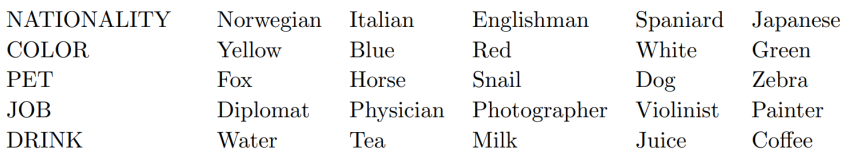
\includegraphics[scale=0.6]{1.2 T42.png}
	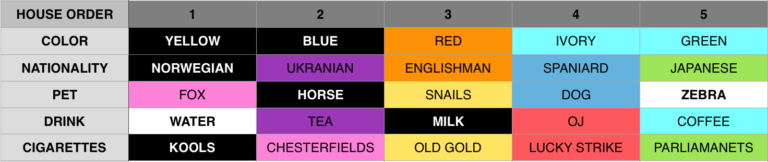
\includegraphics[width=\linewidth]{1.2 T42(2).png}
	\captionof{figure}{}
	In this solution the Japanese man owns the zebra, and the Norwegian drinks water.
\end{Sol}

%---------------------------------------------------------------------------

\clearpage

%---------------------------------------------------------------------------

\begin{tcolorbox}
	[colback=Emerald!10,colframe=cyan!40!black,title=\textbf{Question 45}]
	Find the output of each of these combinatorial circuits.
	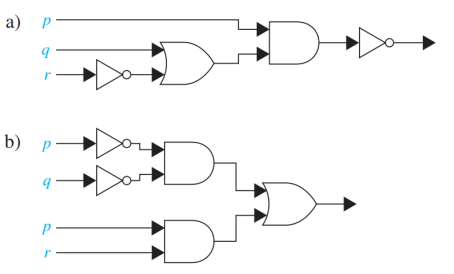
\includegraphics[]{1.2 T45.png}
	\captionof{figure}{}
\end{tcolorbox}
\begin{Sol}[]
	\begin{enumerate}[a)]
		\item $\lnot (p \land (q \lor \lnot r))$
		\item $((\lnot p) \land (\lnot q)) \lor (p \land r)$		
	\end{enumerate}
\end{Sol}

%---------------------------------------------------------------------------

\clearpage

\section{1.3 Propositional Equivalences}

%---------------------------------------------------------------------------

\begin{tcolorbox}
	[colback=Emerald!10,colframe=cyan!40!black,title=\textbf{Question 7}]
	Use De Morgan's laws to find the negation of each of the following statements.
	\begin{enumerate}[a)]
		\item Jan is rich and happy.
		\item Carlos will bicycle or run tomorrow.
		\item Mei walks or takes the bus to class.
		\item Ibrahim is smart and hard working.
	\end{enumerate}
\end{tcolorbox}
\begin{Sol}[]
	\begin{enumerate}[a)]
		\item Jan is not rich or not happy.
		\item Carlos will not bicycle and not run tomorrow.
		\item Mei does not walk and does not take the bus to class.
		\item Ibrahim is not smart or not hard working.
	\end{enumerate}
\end{Sol}

%---------------------------------------------------------------------------

\clearpage

%---------------------------------------------------------------------------

\begin{tcolorbox}
	[colback=Emerald!10,colframe=cyan!40!black,title=\textbf{Question 9}]
	For each of these compound propositions, use the
	conditional-disjunction equivalence (Example 3) to find
	an equivalent compound proposition that does not involve conditionals.
	\begin{enumerate}[a)]
		\item $p \rightarrow \lnot q$
		\item $(p \rightarrow q) \rightarrow r$
		\item $(\lnot q \rightarrow p) \rightarrow (p \rightarrow \lnot q)$
	\end{enumerate}
\end{tcolorbox}
\begin{Sol}[]
	\begin{enumerate}[a)]
		\item $\lnot p \lor q$
		\item $\lnot(p \lor \lnot q) \lor r$
		\item $\lnot(q \lor \lnot p) \lor (\lnot p \lor q)$
	\end{enumerate}
\end{Sol}

%---------------------------------------------------------------------------

\clearpage

%---------------------------------------------------------------------------

\begin{tcolorbox}
	[colback=Emerald!10,colframe=cyan!40!black,title=\textbf{Question 19}]
	Determine whether $(\lnot q \land (p \rightarrow q)) \rightarrow \lnot p$ is a tautology
\end{tcolorbox}
\begin{Sol}[]
	\begin{align}
	(\lnot q \land (p \rightarrow q)) \rightarrow \lnot p &\equiv \lnot (\lnot q \land (\lnot p \lor q)) \lor \lnot p \tag*{by the example 3} \\ 
	&\equiv (q \lor (p \land \lnot q)) \lor \lnot p \tag*{by De Morgan’s laws} \\
	&\equiv ((q \lor p) \land (q \lor \lnot q)) \lor \lnot p \tag*{by Distributive laws} \\
	&\equiv ((q \lor p) \land T) \lor \lnot p \tag*{by Negation laws} \\
	&\equiv (q \lor p) \lor \lnot p \tag*{by Identity laws} \\
	&\equiv q \lor (p \lor \lnot p) \tag*{by Associative laws} \\
	&\equiv q \lor T \tag*{by Negation laws} \\
	&\equiv T \tag*{by Identity laws}
	\end{align}
\end{Sol}

%---------------------------------------------------------------------------

\clearpage

%---------------------------------------------------------------------------

\begin{tcolorbox}
	[colback=Emerald!10,colframe=cyan!40!black,title=\textbf{Question 20}]
	Show that $p \leftrightarrow q$ and $(p \land q) \lor (\lnot p \land \lnot q)$ are logically equivalent.
\end{tcolorbox}
\begin{Sol}[]
	The first proposition is true if and only if \textit{p} and \textit{q} have the same truth value. \\ 
	The second proposition is true if and only if either \textit{p} and \textit{q} are both true, or \textit{p} and \textit{q} are both false \\
	Therefore, the two propositionare are logically equivalent.
\end{Sol}

%---------------------------------------------------------------------------

%---------------------------------------------------------------------------

\begin{tcolorbox}
	[colback=Emerald!10,colframe=cyan!40!black,title=\textbf{Question 21}]
	Show that $\lnot (p \leftrightarrow q)$ and $p \leftrightarrow \lnot q$ are logically equivalent.
\end{tcolorbox}
\begin{Sol}[]
	The first proposition is true if and only if \textit{p} and \textit{q} have different truth values. \\ 
	The second proposition is true if and only if either \textit{p} is true and \textit{q} is false, or \textit{p} is false and \textit{q} is true. \\
	Therefore, the two propositionare are logically equivalent.
\end{Sol}

%---------------------------------------------------------------------------

%---------------------------------------------------------------------------

\begin{tcolorbox}
	[colback=Emerald!10,colframe=cyan!40!black,title=\textbf{Question 22}]
	Show that $p \rightarrow q)$ and $\lnot q \rightarrow \lnot p$ are logically equivalent.
\end{tcolorbox}
\begin{Sol}[]
	The first proposition is false if and only if \textit{p} is true and \textit{q} is false. \\ 
	The second proposition is false if and only if \textit{q} is false and \textit{p} is true \\
	Therefore, the two propositionare are logically equivalent.
\end{Sol}

%---------------------------------------------------------------------------

\clearpage 

%---------------------------------------------------------------------------

\begin{tcolorbox}
	[colback=Emerald!10,colframe=cyan!40!black,title=\textbf{Question 23}]
	Show that $\lnot p \leftrightarrow q$ and  $p \leftrightarrow \lnot q$ are logically equivalent.
\end{tcolorbox}
\begin{Sol}[]
	The first proposition is true if and only if either \textit{p} is true and \textit{q} is false, or \textit{p} is false and \textit{q} is true. \\ 
	The second proposition is true if and only if either \textit{p} is true and \textit{q} is false, or \textit{p} is false and \textit{q} is true. \\
	Therefore, the two propositionare are logically equivalent.
\end{Sol}

%---------------------------------------------------------------------------

%---------------------------------------------------------------------------

\begin{tcolorbox}
	[colback=Emerald!10,colframe=cyan!40!black,title=\textbf{Question 24}]
	Show that $\lnot (p \oplus q)$ and $p \leftrightarrow q$ are logically equivalent.
\end{tcolorbox}
\begin{Sol}[]
	The first proposition is true if and only if \textit{p} and \textit{q} have the same truth value. \\ 
	The second proposition is true if and only if \textit{p} and \textit{q} have the same truth value. \\
	Therefore, the two propositionare are logically equivalent.
\end{Sol}

%---------------------------------------------------------------------------

%---------------------------------------------------------------------------

\begin{tcolorbox}
	[colback=Emerald!10,colframe=cyan!40!black,title=\textbf{Question 25}]
	Show that $\lnot (p \leftrightarrow q)$ and $\lnot p \leftrightarrow q$ are logically equivalent.
\end{tcolorbox}
\begin{Sol}[]
	The first proposition is true if and only if \textit{p} and \textit{q} have different truth values. \\ 
	The second proposition is true if and only if either \textit{p} is true and \textit{q} is false, or \textit{p} is false and \textit{q} is true. \\
	Therefore, the two propositionare are logically equivalent.
\end{Sol}

%---------------------------------------------------------------------------

\clearpage

%---------------------------------------------------------------------------

\begin{tcolorbox}
	[colback=Emerald!10,colframe=cyan!40!black,title=\textbf{Question 26}]
	Show that $ (p \rightarrow q) \land (p \rightarrow r)$ and $p \rightarrow (q \land r)$ are logically equivalent.
\end{tcolorbox}
\begin{Sol}[]
	The first proposition is false if and only if either \textit{p} is true and \textit{q} is false, or \textit{p} is true and \textit{r} is false. \\ 
	The second proposition is false if and only if \textit{p} is true and either \textit{q} is false or \textit{r} is false. \\
	Therefore, the two propositionare are logically equivalent.
\end{Sol}

%---------------------------------------------------------------------------
%---------------------------------------------------------------------------

\begin{tcolorbox}
	[colback=Emerald!10,colframe=cyan!40!black,title=\textbf{Question 27}]
	Show that $ (p \rightarrow r) \land (q \rightarrow r)$ and $(p \lor q) \rightarrow r$ are logically equivalent.
\end{tcolorbox}
\begin{Sol}[]
	The first proposition is false if and only if either \textit{p} is true and \textit{r} is false, or \textit{q} is true and \textit{r} is false. \\ 
	The second proposition is false if and only if either \textit{p} or \textit{q} is true and \textit{r} is false. \\
	Therefore, the two propositionare are logically equivalent.
\end{Sol}

%---------------------------------------------------------------------------

%---------------------------------------------------------------------------

\begin{tcolorbox}
	[colback=Emerald!10,colframe=cyan!40!black,title=\textbf{Question 28}]
	Show that $ (p \rightarrow q) \lor (p \rightarrow r)$ and $p \rightarrow (q \lor r)$ are logically equivalent.
\end{tcolorbox}
\begin{Sol}[]
	The first proposition is false if and only if \textit{p} is true and \textit{q} is false, and \textit{p} is true and \textit{r} is false. \\ 
	The second proposition is false if and only if \textit{p} is true and both \textit{q} and \textit{r} are false. \\
	Therefore, the two propositionare are logically equivalent.
\end{Sol}

%---------------------------------------------------------------------------

\clearpage

%---------------------------------------------------------------------------

\begin{tcolorbox}
	[colback=Emerald!10,colframe=cyan!40!black,title=\textbf{Question 29}]
	Show that $  (p \rightarrow r) \lor (q \rightarrow r)$ and $(p \land q) \rightarrow r$ are logically equivalent.
\end{tcolorbox}
\begin{Sol}[]
	The first proposition is false if and only if \textit{p} is true and \textit{r} is false, and \textit{q} is true and \textit{r} is false. \\ 
	The second proposition is false if and only if either \textit{p} or \textit{q} is true and \textit{r}  is false. \\
	Therefore, the two propositionare are logically equivalent.

\end{Sol}

%---------------------------------------------------------------------------

%---------------------------------------------------------------------------

\begin{tcolorbox}
	[colback=Emerald!10,colframe=cyan!40!black,title=\textbf{Question 30}]
	Show that $ \lnot p \rightarrow (q \rightarrow r)$ and $q \rightarrow (p \lor r) a$ are logically equivalent.
\end{tcolorbox}
\begin{Sol}[]
	The first proposition is false if and only if \textit{p} is false, \textit{q} is true and \textit{r} is false. \\ 
	The second proposition is false if and only if \textit{q} is true and both \textit{p} and \textit{r} are false. \\
	Therefore, the two propositionare are logically equivalent.
\end{Sol}

%---------------------------------------------------------------------------

%---------------------------------------------------------------------------

\begin{tcolorbox}
	[colback=Emerald!10,colframe=cyan!40!black,title=\textbf{Question 31}]
	Show that $p \leftrightarrow q$ and $(p \rightarrow q) \land (q \rightarrow p) $ are logically equivalent.
\end{tcolorbox}
\begin{Sol}[]
	The first proposition is true if and only if \textit{p} and \textit{q} have same truth value. \\ 
	The second proposition is true if and only if \textit{p} is not true when \textit{q} is false, and if \textit{q} is not true when \textit{p} is false. \\
	Therefore, the two propositionare are logically equivalent.
\end{Sol}

%---------------------------------------------------------------------------

\clearpage

%---------------------------------------------------------------------------

\begin{tcolorbox}
	[colback=Emerald!10,colframe=cyan!40!black,title=\textbf{Question 32}]
	Show that $ p \leftrightarrow q$ and $\lnot p \leftrightarrow \lnot q$ are logically equivalent.
\end{tcolorbox}
\begin{Sol}[]
	The first proposition is true if and only if \textit{p} and \textit{q} have same truth value. \\ 
	The second proposition is true if and only if $\lnot p$ and $\lnot q$ have same truth value,  equivalent to \textit{p} and \textit{q} have same truth value. \\
	Therefore, the two propositionare are logically equivalent.
\end{Sol}

%---------------------------------------------------------------------------

%---------------------------------------------------------------------------

\begin{tcolorbox}
	[colback=Emerald!10,colframe=cyan!40!black,title=\textbf{Question 33}]
	Show that $ (p \rightarrow q) \land (q \rightarrow r) \rightarrow (p \rightarrow r) $ is a tautology.
\end{tcolorbox}
\begin{Sol}[]
	We can construct a truth table. \\ \\
	\begin{tabular}{|p{2cm}|p{2cm}|p{2cm}|p{6cm}}
		\makecell[c]{$p$} & \makecell[c]{$q$} & \makecell[c]{$r$} & \makecell[c]{$ (p \rightarrow q) \land (q \rightarrow r) \rightarrow (p \rightarrow r)$}\\
		\makecell[c]{T}& \makecell[c]{T}& \makecell[c]{T}& \makecell[c]{T}\\
		\makecell[c]{T}& \makecell[c]{T}& \makecell[c]{F}& \makecell[c]{T}\\
		\makecell[c]{T}& \makecell[c]{F}& \makecell[c]{T}& \makecell[c]{T}\\
		\makecell[c]{T}& \makecell[c]{F}& \makecell[c]{F}& \makecell[c]{T}\\
		\makecell[c]{F}& \makecell[c]{T}& \makecell[c]{T}& \makecell[c]{T}\\
		\makecell[c]{F}& \makecell[c]{T}& \makecell[c]{F}& \makecell[c]{T}\\
		\makecell[c]{F}& \makecell[c]{F}& \makecell[c]{T}& \makecell[c]{T}\\
		\makecell[c]{F}& \makecell[c]{F}& \makecell[c]{F}& \makecell[c]{T}\\
	\end{tabular}
	\\ \\The last column is all Ts.
\end{Sol}

%---------------------------------------------------------------------------

\clearpage

%---------------------------------------------------------------------------

\begin{tcolorbox}
	[colback=Emerald!10,colframe=cyan!40!black,title=\textbf{Question 46}]
	Suppose that a truth table in n propositional variables is
	specified. Show that a compound proposition with this
	truth table can be formed by taking the disjunction of
	conjunctions of the variables or their negations, with one
	conjunction included for each combination of values for
	which the compound proposition is true. The resulting
	compound proposition is said to be in disjunctive normal form.
	\\ A collection of logical operators is called functionally complete if every compound proposition is logically equivalent
	to a compound proposition involving only these logical operators.
\end{tcolorbox}
\begin{Sol}[]
	For each line of truth table, we can write down a conjunction of \textit{n} propositional variables corresponds to this case. Only when these atomic propositions takes the corresponding truth value of this line that the conjunction can be true. \\
	If we pick the lines of truth table that make the compound proposition true, and write down their conjunctions,  and take the disjunction of the resulting propositions,
	then we have the proposition in its disjunctive normal form.
\end{Sol}

%---------------------------------------------------------------------------


\clearpage

%---------------------------------------------------------------------------

\begin{tcolorbox}
	[colback=Emerald!10,colframe=cyan!40!black,title=\textbf{Question 50}]
	Construct a truth table for the logical operator \textit{NAND}.
\end{tcolorbox}
\begin{Sol}[]
	\begin{tabular}{|p{2cm}|p{2cm}|p{4cm}}
		\makecell[c]{$p$} & \makecell[c]{$q$} &\makecell[c]{ $p\ \vert \ q$ } \\
		\makecell[c]{T}& \makecell[c]{T}& \makecell[c]{T}\\
		\makecell[c]{T}& \makecell[c]{F}& \makecell[c]{F}\\
		\makecell[c]{F}& \makecell[c]{T}& \makecell[c]{F}\\
		\makecell[c]{F}& \makecell[c]{F}& \makecell[c]{F}
	\end{tabular}
\end{Sol}

%---------------------------------------------------------------------------

%---------------------------------------------------------------------------

\begin{tcolorbox}
	[colback=Emerald!10,colframe=cyan!40!black,title=\textbf{Question 51}]
	Show that $p\ \vert \ q$ is logically equivalent to $\lnot (p \land q)$.
\end{tcolorbox}
\begin{Sol}[]
	$\lnot (p \land q)$ is false if and only if either $p$ or $q$, or both, are false
	,this was the definition of $p\ \vert \ q$ , the two are logically
	equivalent.
\end{Sol}

%---------------------------------------------------------------------------

\clearpage

%---------------------------------------------------------------------------

\begin{tcolorbox}
	[colback=Emerald!10,colframe=cyan!40!black,title=\textbf{Question 52}]
	Construct a truth table for the logical operator \textit{NOR}.
\end{tcolorbox}
\begin{Sol}[]
	\begin{tabular}{|p{2cm}|p{2cm}|p{4cm}}
		\makecell[c]{$p$} & \makecell[c]{$q$} &\makecell[c]{ $p \downarrow  q$ } \\
		\makecell[c]{T}& \makecell[c]{T}& \makecell[c]{F}\\
		\makecell[c]{T}& \makecell[c]{F}& \makecell[c]{F}\\
		\makecell[c]{F}& \makecell[c]{T}& \makecell[c]{F}\\
		\makecell[c]{F}& \makecell[c]{F}& \makecell[c]{T}
	\end{tabular}
\end{Sol}

%---------------------------------------------------------------------------

%---------------------------------------------------------------------------

\begin{tcolorbox}
	[colback=Emerald!10,colframe=cyan!40!black,title=\textbf{Question 53}]
	Show that $p \downarrow  q$ is logically equivalent to $\lnot(p \lor q)$.
\end{tcolorbox}
\begin{Sol}[]
	$\lnot(p \lor q)$ is true when both p and q are false, and is false otherwise.
	Because this was the definition of $p \downarrow  q$ , the two are logically
	equivalent.
\end{Sol}

%---------------------------------------------------------------------------

%---------------------------------------------------------------------------

\begin{tcolorbox}
	[colback=Emerald!10,colframe=cyan!40!black,title=\textbf{Question 57}]
	 Show that $p\ \vert \ q$ and $q\ \vert \ p$ are equivalent.
\end{tcolorbox}
\begin{Sol}[]
	From the truth table of Question 50, we can proof that $p\ \vert \ q$ and $q\ \vert \ p$ are equivalent.
\end{Sol}

%---------------------------------------------------------------------------
\end{document}